I will explore here more technical details on the design and calibration explored as part of this project and necessary to extracting scientific information from the IRVB.

\section{Issues of the IRVB implementation in MU01}\label{Issues of the IRVB implementation in MU01}

It was realised when the data from super- experiment was analysed that the LOS that enter the super-X chamber have all a similar path through it, causing a large uncertainty on the source of the emissivity there. This can be shown by placing a phantom with known emissivity in the super-x chamber, determining the power on the foil and invert back to the emissivity. The result is shown in \autoref{fig:sxd_bad}.

\begin{figure}
     \centering
     \begin{subfigure}{0.45\textwidth}
         \centering
         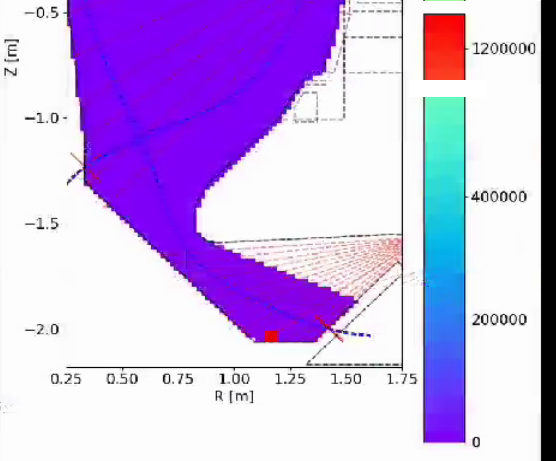
\includegraphics[trim={0 0 30 0},clip,width=\textwidth]{Chapters/appendix1/figs/phantom_sdx.png}
         %\caption{SXD 45239}
         %\label{fig:table45239}
     \end{subfigure}
     \hfill
     \begin{subfigure}{0.45\textwidth}
         \centering
         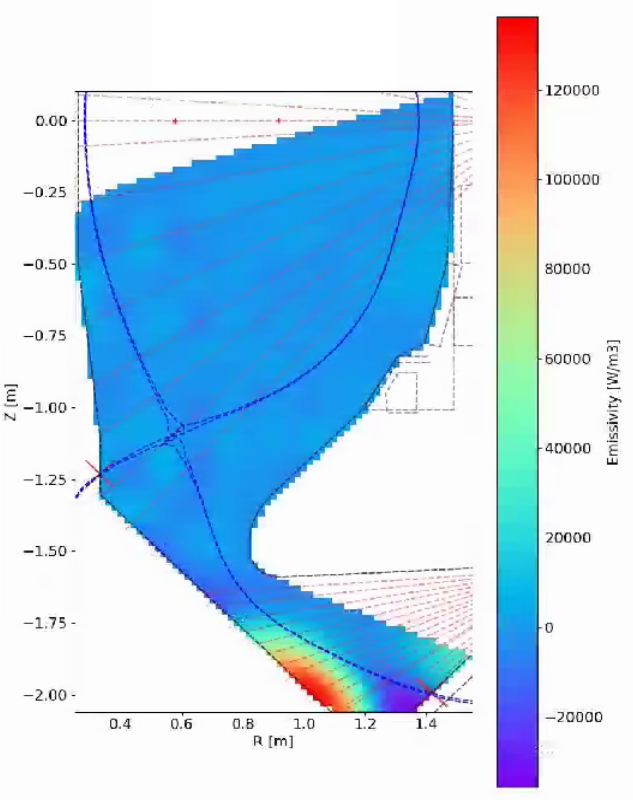
\includegraphics[width=\textwidth]{Chapters/appendix1/figs/inversion_sdx.png}
         %\caption{CD 45401}
         %\label{fig:table45401}
     \end{subfigure}

    \caption{Phantom of radiation localised in the SXD and tomographically inverted emissivity, showing that the present setup is unable to reconstruct detailed emissivity maps of the radiation in the SXD.}
    \label{fig:sxd_bad}
\end{figure}


The inversion routine cannot locate the source of the emission, but the total radiated power in the chamber is still within $\approx 30\%$ of the input.

\subsection{MU02 geometry optimisation}

After the results of the first MASTU campaign it was clear that with appropriate binning the SNR for relatively weak ohmic discharges is large enough (with binning of 14 temporal steps, 7 per digitizer, and 3x3 spatial peak signal on the foil $\approx 40W/m^2$ with uncertainty \hl{$\approx 7W/m^2$}) for high resolution emissivity maps. One negative result is that, because of the small angular difference between the different lines of sights (LOSs) entering the super-x chamber the resolution there is insufficient to reconstruct an emissivity map.
To define the optimal geometry for good SNR two test cases were found:
\begin{itemize}
    \item a ohmic SXD discharge with weak widespread radiation with the purpose of reconstructing the broad characteristics but mostly the total and partial sums of the radiated power. I decided to use 45239 at t=493ms
    \item a conventional high power H-mode discharge from a strong density scan and with x-point radiator, with strong signal, for the purpose of accurately reconstruct the radiation around the x-point. I decided to use 45401 at t=714ms
\end{itemize}

To perform the comparison the emissivity phantoms were calculated for each case with a binning of 14 temporal steps, 7 per camera digitizer, and 3x3 spatial ones with the present geometry. The negative emissivity was set to 0; to recreate a more realistic (field aligned) emissivity profile the emissivity was set to zero at $r>1m$ and $z>-1.5m$ for the 45239 phantom, while at $r>1m$ for 45401. The phantoms created are shown in \autoref{fig:phantoms}. The black dashed lines show the regions that will be used to compare the results.

\begin{figure}
     \centering
     \begin{subfigure}{0.45\textwidth}
         \centering
         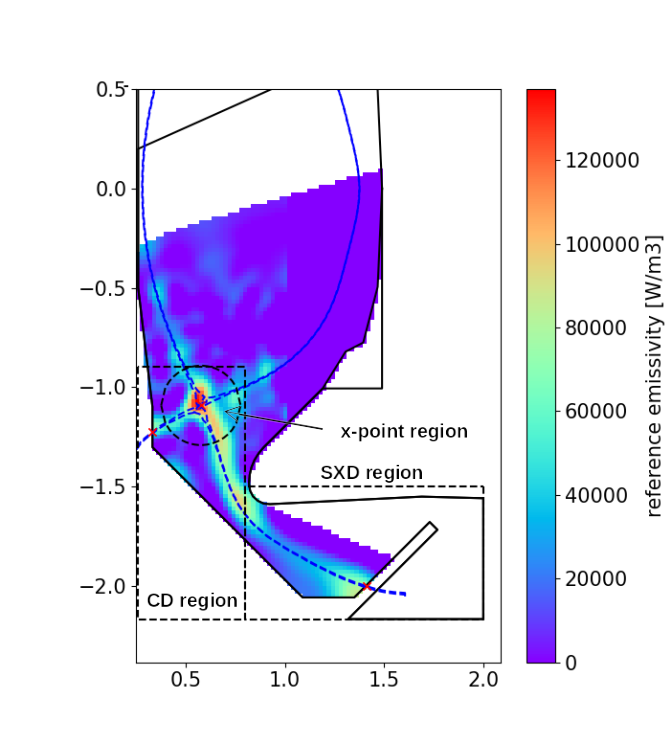
\includegraphics[trim={70 20 0 20},clip,width=\textwidth]{Chapters/appendix1/figs/45239_2.png}
         \caption{SXD 45239}
         \label{fig:45239}
     \end{subfigure}
     \hfill
     \begin{subfigure}{0.45\textwidth}
         \centering
         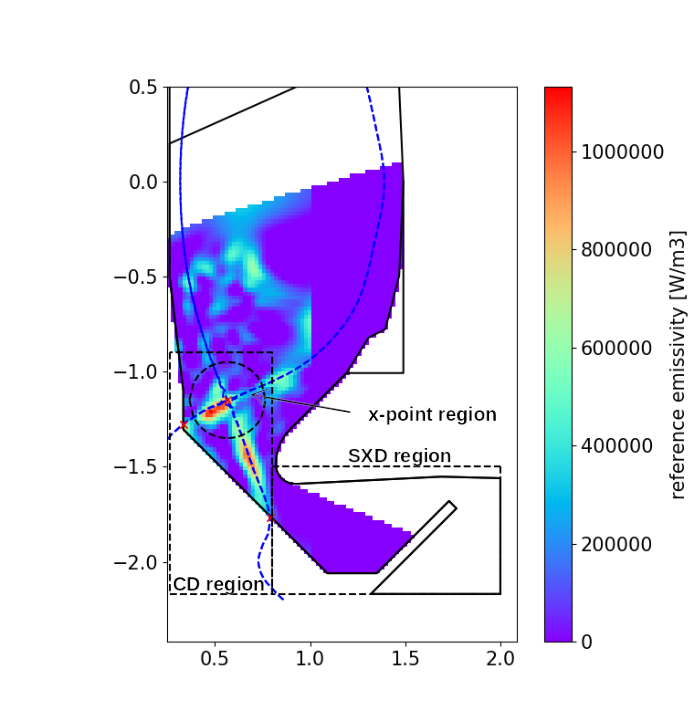
\includegraphics[trim={70 20 0 20},clip,width=\textwidth]{Chapters/appendix1/figs/45401_2.png}
         \caption{CD 45401}
         \label{fig:45401_app}
     \end{subfigure}

    \caption{Phantoms used to compare the effect of different geometries on the tomographic inversion process. Left: shot 45239, 493ms, SXD discharge, emissivity=0 at $r>1m$ and $z>-1.5m$. Right:  shot 45401, 714ms, CD discharge, emissivity=0 at $r>1m$. The dashed lines represent the regions over which the results will be compared.}
    \label{fig:phantoms}
\end{figure}

The configurations investigated are all combinations of 45 and 60mm standoff and 4 and 6mm pinhole. 
For each configuration the geometry matrix is calculated using CHERAB to obtain the power absorbed by the foil. The temperature was then calculated with the same phantom for a number of time steps equal to 4 times the binning and the count noise added. The temperature profile is then binned and the power to the foil is calculated. The tomographic inversion is performed with the intermediate time step to find the new emissivity profile. The profiles are compared to the phantom in terms of local emissivity and integrated power. The results are shown in \autoref{fig:table_mu02}.

\begin{figure}
     \centering
     \begin{subfigure}{0.45\textwidth}
         \centering
         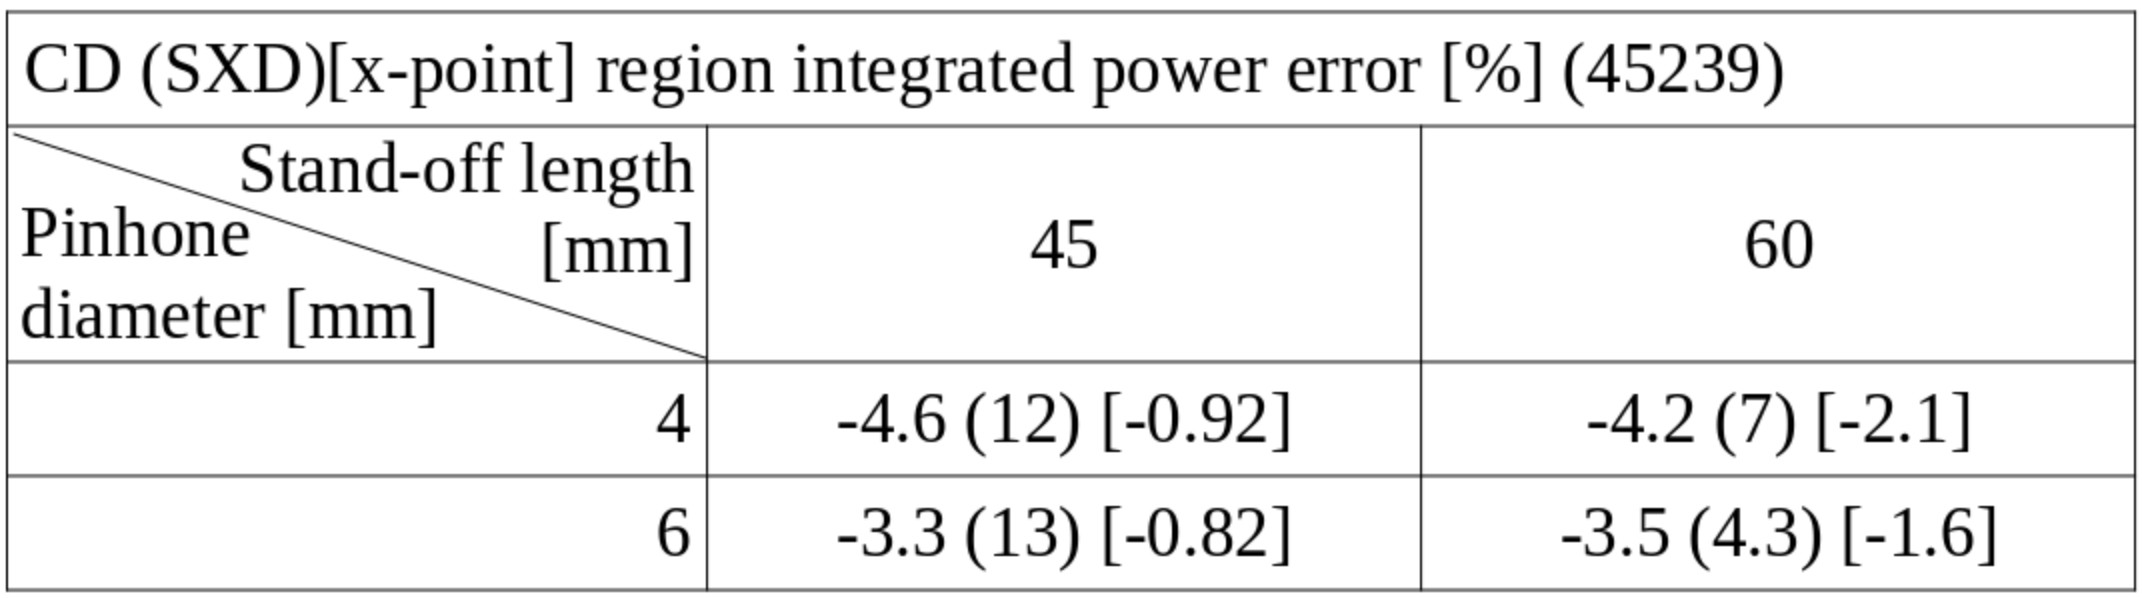
\includegraphics[width=\textwidth]{Chapters/appendix1/figs/table45239.png}
         \caption{SXD 45239}
         \label{fig:table45239}
     \end{subfigure}
     \hfill
     \begin{subfigure}{0.45\textwidth}
         \centering
         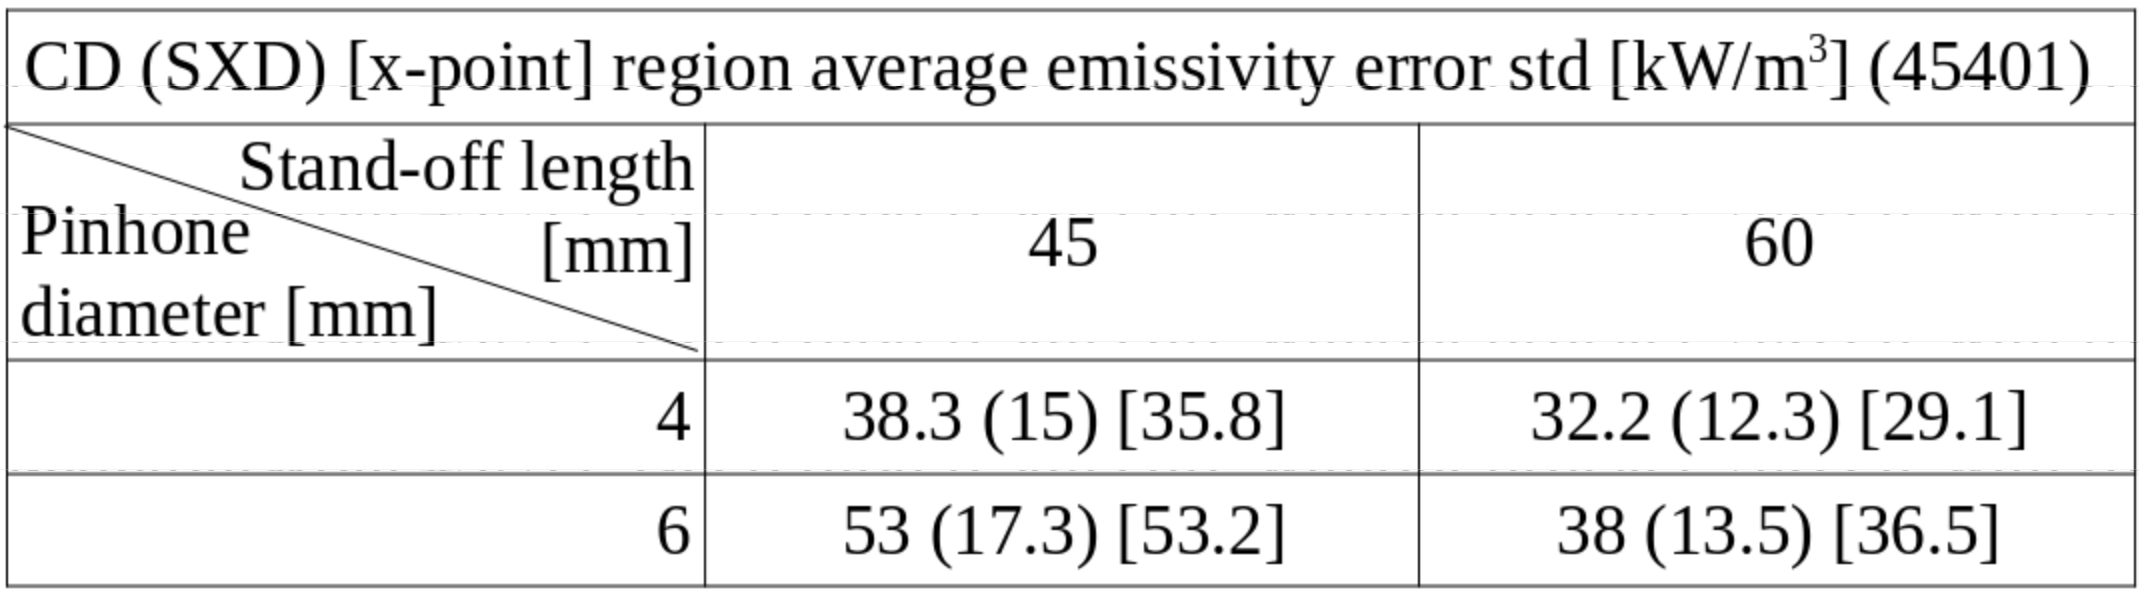
\includegraphics[width=\textwidth]{Chapters/appendix1/figs/table45401.png}
         \caption{CD 45401}
         \label{fig:table45401}
     \end{subfigure}

    \caption{Comparison of the integrated power $\%$ error for all geometric configurations for the SXD phantom from 45239 (a) and of the averaged power error std for all geometric configurations for the CD phantom from 45401 (b). CD region results are without bracket, SXD in with round brackets and x-point ones with square brackets}
    \label{fig:table_mu02}
\end{figure}

A larger pinhole allows a more precise accounting of the integrated power. Given the present SNR though, the improvement is minor. This is even more true considering that in MU02 the discharges are expected to be more energetic, with beam power even in L-mode. The power accounting in the SXD also improves with a longer stand-off.
The 60mm stand-off 4mm pinhole diameter configuration yields the better performance in terms of resolution around the x-point with strong signal. For high SNR additional LOSs count more than an even stronger signal.

Regarding the loss of spatial resolution in the SXD the stonger the signal the better. For larger pinhole the reconstructed radiation is more localised but still elongated along the LOS. Considering the design of IRVB aimed at a high resolution around the x-point and not the SXD, this is considered less important. It will be important to remember that the data inside the SXD is useful for integrated measurements rather than profiles.
With these consideration it was decided to adopt the 4mm diameter pinhole and 60mm long stand-off. It is the solution that causes the lower signal strength, but it is still deemed sufficient.

\section{IRVB calibration}\label{IRVBcalibration}


\subsection{counts oscillation suppression}
not sure if this is necessary
\subsection{geometry matrix: CHERAB}
not sure if this is necessary